% !TEX root = ../../main.tex

\section{Optimisations et performances}
\label{s:3:info}

Cette section s'intéresse aux aspects techniques de l'implémentation des schémas présentés dans la section~\ref{sec:3:scheme}. Il sera tout d'abord question de méthode de génération de code, utilisée uniquement dans le cadre de la méthode de Lawson, puis nous discuterons des performances et des choix d'implémentation effectués.

\subsection{Génération automatique de code}
\label{ssec:3:codegen}

La simulation d'un système à 7 inconnues, dont 1 inconnue à 4 dimensions, avec une méthode de type Lawson-Runge-Kutta (LRK) d'ordre élevé, nécessite de nombreuses lignes de code dont l'écriture peut s'avérer fastidieuse, entrainant de nombreuses possibilités de bugs informatiques. Une part importante de l'analyse ayant été réalisée à l'aide de la bibliothèque de calcul symbolique \Python{} : \sympy, il a été décidé de poursuivre son utilisation pour aider à l'écriture du code de simulation. Dans un premier temps cet usage s'est limité à une aide à l'écriture en générant chacune des 7 expressions pour chaque variable, et ce à chaque étage de la méthode LRK (3 étages pour RK(3,3), jusqu'à 5 étages pour une méthode comme DP4(3)). Des outils de méta-programmation, développés en \Python{}, ont été utilisés pour obtenir une génération complète du code à partir d'un squelette de code \CC{} et de l'écriture mathématique du schéma LRK que l'utilisateur souhaite utiliser.

Les expressions \sympy{} sont gérées comme des arbres syntaxiques dont les feuilles sont des nombres ou des symboles. Ces derniers vont servir à représenter des variables \CC, il est donc nécessaire dans un premier temps de s'assurer que la conversion de ces symboles en chaînes de caractères assure des noms de variables valide en \CC. En effet il est fréquent d'utiliser des symboles s'exportant facilement en \LaTeX{}, or un tel symbole n'est pas utilisable de la sorte comme nom de variable ; par exemple $\Delta t$ s'exportera par défaut en chaîne de caractères en "\texttt{\textbackslash Delta\textbackslash\ t}". Les nœuds de l'arbre syntaxique sont des fonctions, il y a alors deux cas à distinguer. Soit il s'agit d'une fonction dont la représentation en \Python{} est la même qu'en \CC, auquel cas aucune opération particulière n'est nécessaire ; c'est le cas par exemple des opérations arithmétiques $+$, $-$, $\times$ et $\divisionsymbol$ qui sont représentées par les opérateurs binaires \texttt{+}, \texttt{-}, \texttt{*} et \texttt{/} en \Python{} et \CC{}. Soit il s'agit d'une fonction dont la représentation \Python{} et \CC{} diffère, auquel cas il est nécessaire de créer une fonction \sympy{} qui aura le même nom que la fonction \CC{} associée, et de substituer le nœud de l'arbre syntaxique par cette nouvelle fonction. La conversion en chaîne de caractère de l'arbre ainsi modifié sera une expression \CC{} valide. Il est possible d'améliorer l'expression \CC{} en faisant une évaluation numérique des nombres rationnels (et potentiellement aussi irrationnels) présents, pour limiter le nombre d'opérations dans l'expression finale. Ainsi l'expression \texttt{1/3} sera substituée par \texttt{0.333333333333333}, cela permet d'éviter des interprétations de fractions comme des divisions entières par le compilateur.

Pour chaque étage de la méthode LRK, il est ainsi possible d'obtenir une expression \CC{} valide par variable. L'étape supplémentaire est d'utiliser un moteur de \emph{template} pour insérer ces expressions dans un squelette de code qui s'adapte automatiquement au nombre d'étages de la méthode LRK, en initialisant et allouant les variables temporaires nécessaires. Ce travail est effectué par le moteur de \emph{template} Jinja2, qui est une bibliothèque \Python{} permettant d'ajouter des opérations logiques en plus d'une simple substitution de champs dans un squelette de code préexistant. Le squelette en pseudo-code d'un étage d'une méthode LRK est donné en exemple dans l'algorithme~\ref{alg:squeltte} dans la section~\ref{ssec:3:stage}.

\paragraph{Nota Bene :} La bibliothèque \sympy{} contient des fonctions permettant la génération de code en C ou Fortran, mais le fonctionnement de celles-ci s'adapte mal à une intégration dans une boucle d'un code déjà existant. De plus les fonctions ainsi générées ne fonctionnent pas avec un code contenant des \emph{template} \CC, pour changer éventuellement de type pour de possibles optimisations. Elles ne prennent en paramètre que des valeurs par copie ou par pointeur, ce qui limite leur usage avec des structures de données évoluées proposées par les librairies \CC. Il serait envisageable d'utiliser certains des mécanismes présents dans ces fonctions pour améliorer la génération de code proposé ci-dessus, en utilisant un parcours d'arbre syntaxique pour construire un \emph{Abstract Syntax Tree} (AST) permettant la génération dans n'importe quel langage d'une expression. Les fonctions \sympy{} de génération de code sont encore en phase de développement et ne disposent pas d'une documentation complète. Les outils mis en place au cours de cette thèse pallient certains problèmes de \sympy{}, mais ne sont adaptés qu'à ce contexte précis.

\subsection{Performances}

Nous souhaitons dans cette section présenter les choix techniques effectués pour garantir la performance de l'implémentation des schémas détaillés dans la section~\ref{sec:3:scheme}. Nous essayerons aussi de quantifier cette performance sur le code séquentiel. Une parallélisation à l'aide d'OpenMP a été envosagée mais non mise en place à cause de la bibliothèque de calcul des FFT utilisée, nécessitant une prise en charge particulière de celles-ci.

\subsubsection{Structure de données}

Le choix a été fait, durant toute cette thèse, d'utiliser une méthode spectrale pour résoudre le transport en espace (direction $x$ ou $z$). Cela implique d'effectuer régulièrement des transformées de Fourier, ou des transformées inverses. Pour effectuer ces opérations efficacement il est nécessaire que cette mémoire soit contigüe, cela indique qu'il s'agit du dernier indice dans les tableaux manipulés en \CC. La méthode WENO5, utilisée en vitesse, nécessite le \emph{stencil} représenté sur la figure~\ref{fig:3:stencil}. Mais cette représentation est trompeuse, en effet les différents points représentés ne sont pas contigus en mémoire, et les points $f_{[k_x,k_y,k_z,i]}$ et $f_{[k_x+1,k_y,k_z,i]}$, par exemple, sont distants de $N_z\times N_{v_z} \times N_{v_y} + 1$ cases mémoires ; la mémoire étant d'abord contigüe en $z$, puis $v_z$, $v_y$ et enfin $v_x$. Ainsi l'accès aux cases mémoires de ce \emph{stencil} est coûteux, conclusion confirmée par une étude à l'aide d'outils de profilage de code telle que le module Massif de Valgrind.

\begin{figure}
  \centering
  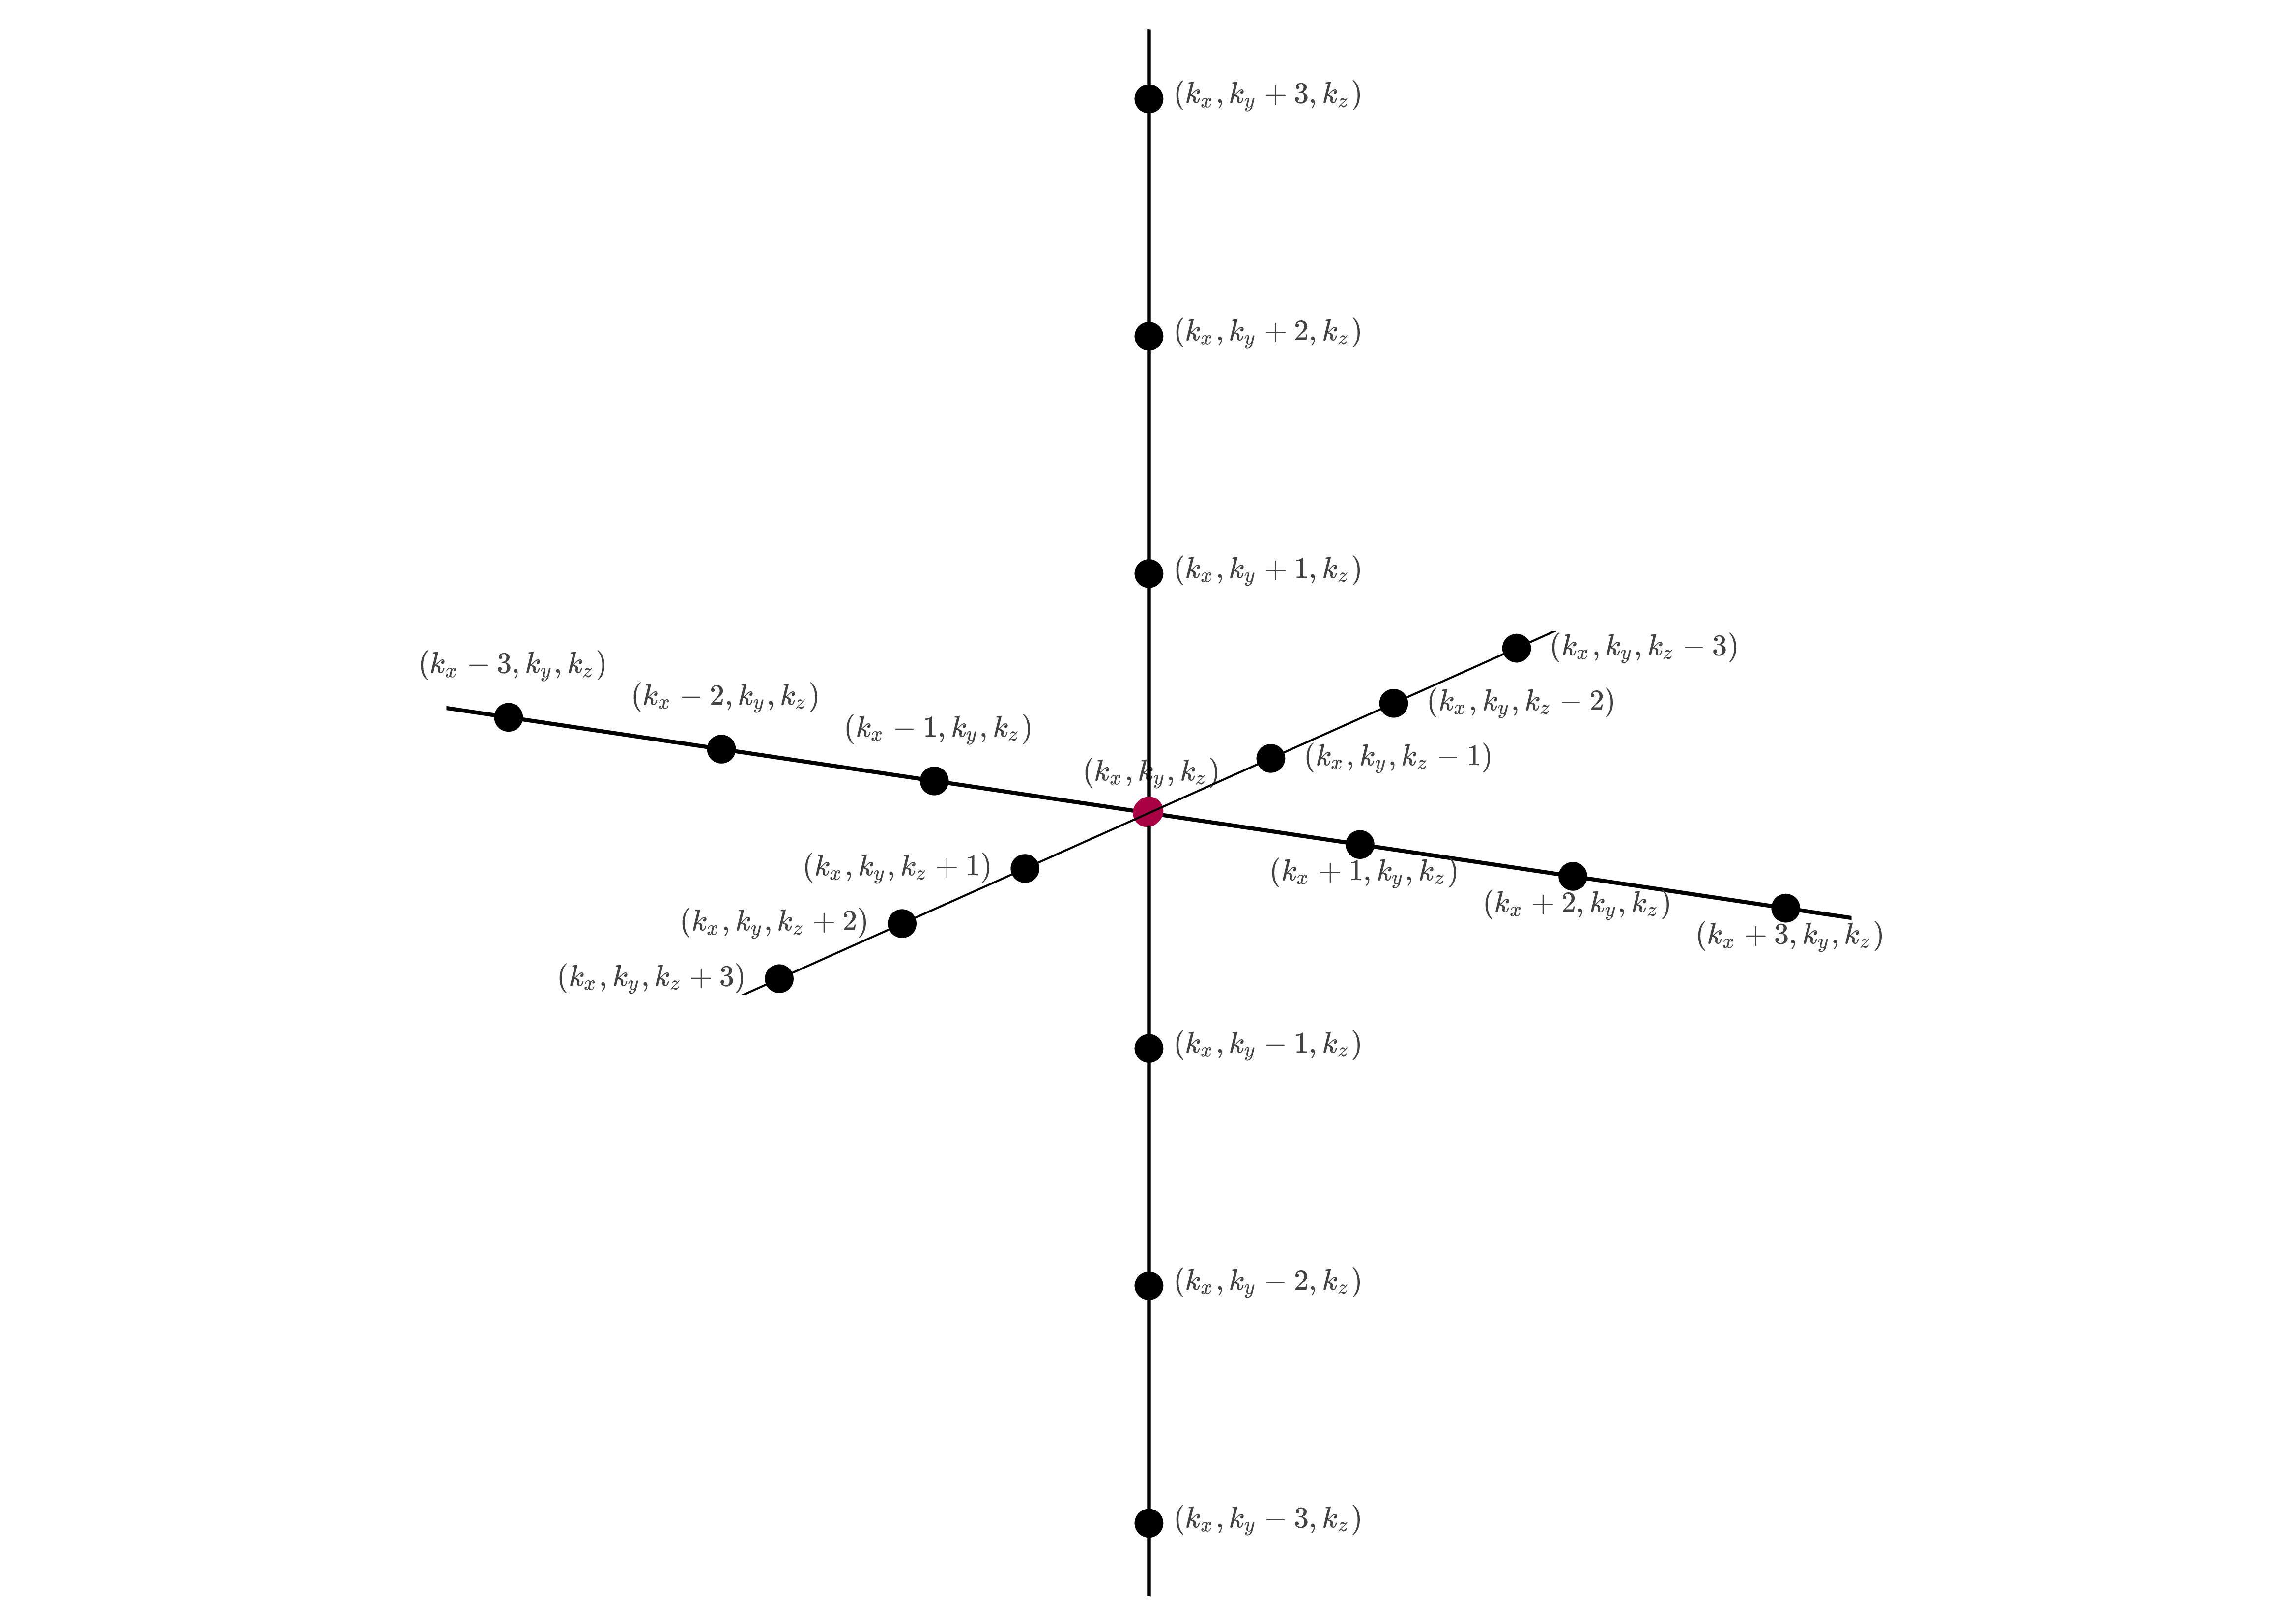
\includegraphics[width=0.75\textwidth]{\localPath/figures/stencil}
  \caption{Représentation à 3 dimensions du \emph{stencil}, centré sur le point $(k_x,k_y,k_z)$, de la méthode WENO5 utilisée pour résoudre le terme $(\vb{E}+\vb{v}\times\vb{B})\cdot\nabla_{\vb{v}}f$.}
  \label{fig:3:stencil}
\end{figure}

Cette structure est imposée par les différentes transformées de Fourier et transformées inverses effectuées dans la direction $z$ dans notre méthode de résolution, et est commune à la fois aux méthodes de \emph{splitting} et de Lawson. S'affranchir de transformées de Fourier (en restant dans l'espace complexe ou non) permettrait de structurer nos données selon une courbe d'Hilbert qui préserve bien la localité des données, rendant les accès mémoire aux données de ce \emph{stencil} moins coûteux.

\subsubsection{Performance séquentielle}

Le cadre multi-dimensionnel se prête moins au raffinement du maillage ou à de nombreux tests pour effectuer des mesures fines du pas de temps. Un test a tout de même été effectué avec toutes les simulations stables numériquement sur le maillage $N_z \times N_{v_x} \times N_{v_y} \times N_{v_z}=27\times32\times32\times41$ et avec un pas de temps constant $\Delta t=0.05$. Les temps de calcul sont présentés dans le tableau~\ref{tab:3:computing:time}, avec l'ajout de deux méthodes à pas de temps adaptatif (LDP4(3) et LDP4(3) - $P_{2,2}$) pour lesquelles le pas de temps $\Delta t=0.05$ n'est que le pas de temps initial. On remarque que l'approximation de l'exponentielle de la partie linéaire d'une méthode de Lawson, avec une série de Taylor ou un approximant de Padé, n'introduit pas de coût visible sur le temps de calcul. On remarque même un temps de calcul plus faible, qui peut être dû au coût de calcul de la fonction \texttt{std::exp}\footnote{La fonction \CC{} \texttt{std::exp} est la fonction exponentielle de la bibliothèque standard de \CC{}.}, utilisée dans les méthodes de Lawson exactes, par rapport à l'évaluation de fractions rationnelles nécessaires dans les méthodes de Lawson couplées à une série de Taylor ou un approximant de Padé.

\begin{table}[h]
  \centering
  \begin{tabular}{l|r}
    Méthode & temps de calcul \\
    \hline
    Méthode de Lie       &                $13\,\textrm{h}\ 25\,\textrm{min}\ 10\,\textrm{s}$ \\
    Méthode de Strang    &                $17\,\textrm{h}\ 09\,\textrm{min}\ 54\,\textrm{s}$ \\
    Méthode de Suzuki    & $3\,\textrm{j}\ 03\,\textrm{h}\ 05\,\textrm{min}\ 24\,\textrm{s}$ \\
    \hline
    LRK(3,3)             &                $11\,\textrm{h}\ 29\,\textrm{min}\ 09\,\textrm{s}$ \\
    LRK(3,3) - $T_4$     &                $10\,\textrm{h}\ 53\,\textrm{min}\ 40\,\textrm{s}$ \\
    LRK(3,3) - $P_{1,1}$ &                $10\,\textrm{h}\ 54\,\textrm{min}\ 11\,\textrm{s}$ \\
    LRK(3,3) - $P_{2,2}$ &                $10\,\textrm{h}\ 55\,\textrm{min}\ 26\,\textrm{s}$ \\
    \hline
    LRK(4,4)             &                $14\,\textrm{h}\ 06\,\textrm{min}\ 15\,\textrm{s}$ \\
    LRK(4,4) - $T_5$     &                $14\,\textrm{h}\ 00\,\textrm{min}\ 03\,\textrm{s}$ \\
    LRK(4,4) - $P_{2,2}$ &                $13\,\textrm{h}\ 59\,\textrm{min}\ 59\,\textrm{s}$ \\
    \hline
    LDP4(3)              &                $11\,\textrm{h}\ 44\,\textrm{min}\ 04\,\textrm{s}$ \\
    LDP4(3) - $P_{2,2}$  &                $04\,\textrm{h}\ 09\,\textrm{min}\ 44\,\textrm{s}$ \\
  \end{tabular}
  \caption{Temps de calcul pour les différentes simulations avec le maillage $N_z \times N_{v_x} \times N_{v_y} \times N_{v_z}=27\times32\times32\times41$ et le pas de temps $\Delta t = 0.05$ (pas de temps initial pour les deux simulations à pas de temps adaptatif).}
  \label{tab:3:computing:time}
\end{table}

Pour comparer également la qualité des résultats, en plus de leur vitesse d'obtention, nous traçons sur la figure~\ref{fig:3:H_time} l'erreur relative sur l'énergie totale pour différentes simulations. Pour la visibilité de la courbe, nous ne conservons ici que les simulations obtenues avec les méthodes de Strang, de Suzuki ainsi que les méthodes de Lawson LRK(4,4) et LDP4(3) couplées avec l'approximant de Padé $P_{2,2}$. On remarque que les méthodes géométriques (méthodes de Strang et de Suzuki), à cause du maillage trop grossier, n'ont pas le comportement attendu, c'est-à-dire une oscillation autour de zéro. La méthode de Strang, comme la méthode de Lie, donne une erreur relative bien plus intéressante ($5.1\%$) que la méthode de Suzuki ($12.1\%$). Les méthodes de Lawson donnent des erreurs relatives similaires, c'est-à-dire autour de $8.4\%$, c'est principalement le temps de calcul qui distingue ces différentes méthodes, et non la précision de leurs résultats, même pour les méthodes de Lawson d'ordre 3. L'impact faible de l'ordre de la méthode sur les résultats vient du maillage relativement grossier.

\begin{figure}
  \centering
  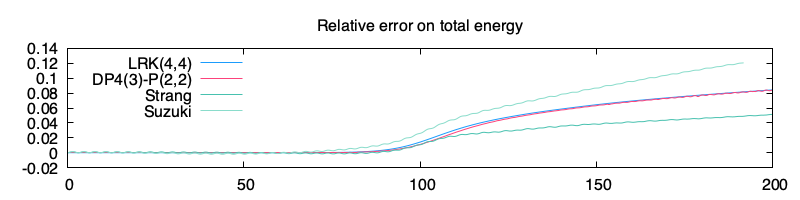
\includegraphics[width=\textwidth]{\localPath/figures/H_time.png}
  \caption{Comparaison de l'erreur relative au cours du temps pour différentes simulations : méthode de Strang, Suzuki, de Lawson $LRK(4,4)$ et la méthode de Lawson à pas de temps adaptatif couplée à un approximant de Padé $LDP4(3)-P_{2,2}$.}
  \label{fig:3:H_time}
\end{figure}

%\subsubsection{Performance parallélisée}


